\documentclass[a4paper]{article}

\usepackage{url}
\usepackage{graphicx}	% For figure environment
\usepackage{epstopdf}
\usepackage[center]{subfigure}
\usepackage{amssymb}	% For mathematical figures like \mathbb{R}
\usepackage{amsmath}
\usepackage{framed}
\usepackage{tikz}
\usetikzlibrary{mindmap,trees}
\usepackage{pdflscape}
\usepackage[a4paper]{geometry}
\usepackage{subfiles}


\title{Advanced Systems Lab - Milestone I} 
\author{Lukas Elmer, Matthias Ganz} 
\date{\today} 


\begin{document}

\maketitle


\begin{abstract}

This document, describes the message queuing system which was build. Architecture and design choices are shown and explained. Further test scenarios and test loads are defined. Resulting test output is described and analysed.

\end{abstract}

%% %%%%%%%%%%%%%%%%%%%%%%%%%%%%%%%%%%%%%%%%%%%%%%
\section{Messaging System}
In this section the system under test (also named as \textbf{middle ware}  or \textbf{broker}) is described.


%% ----------------------------------------------
\subsection{Overview}

Figure \ref{fig:system-overview} shows a generic setup of the messaging system. Multiple middle ware components are connected to a single database and severs a couple of clients. Application state is persisted on the database, therefore a middle ware component can be considered as stateless.

% ------------------------------------------------
% Figure - system overview

\begin{figure}
  \begin{center}
    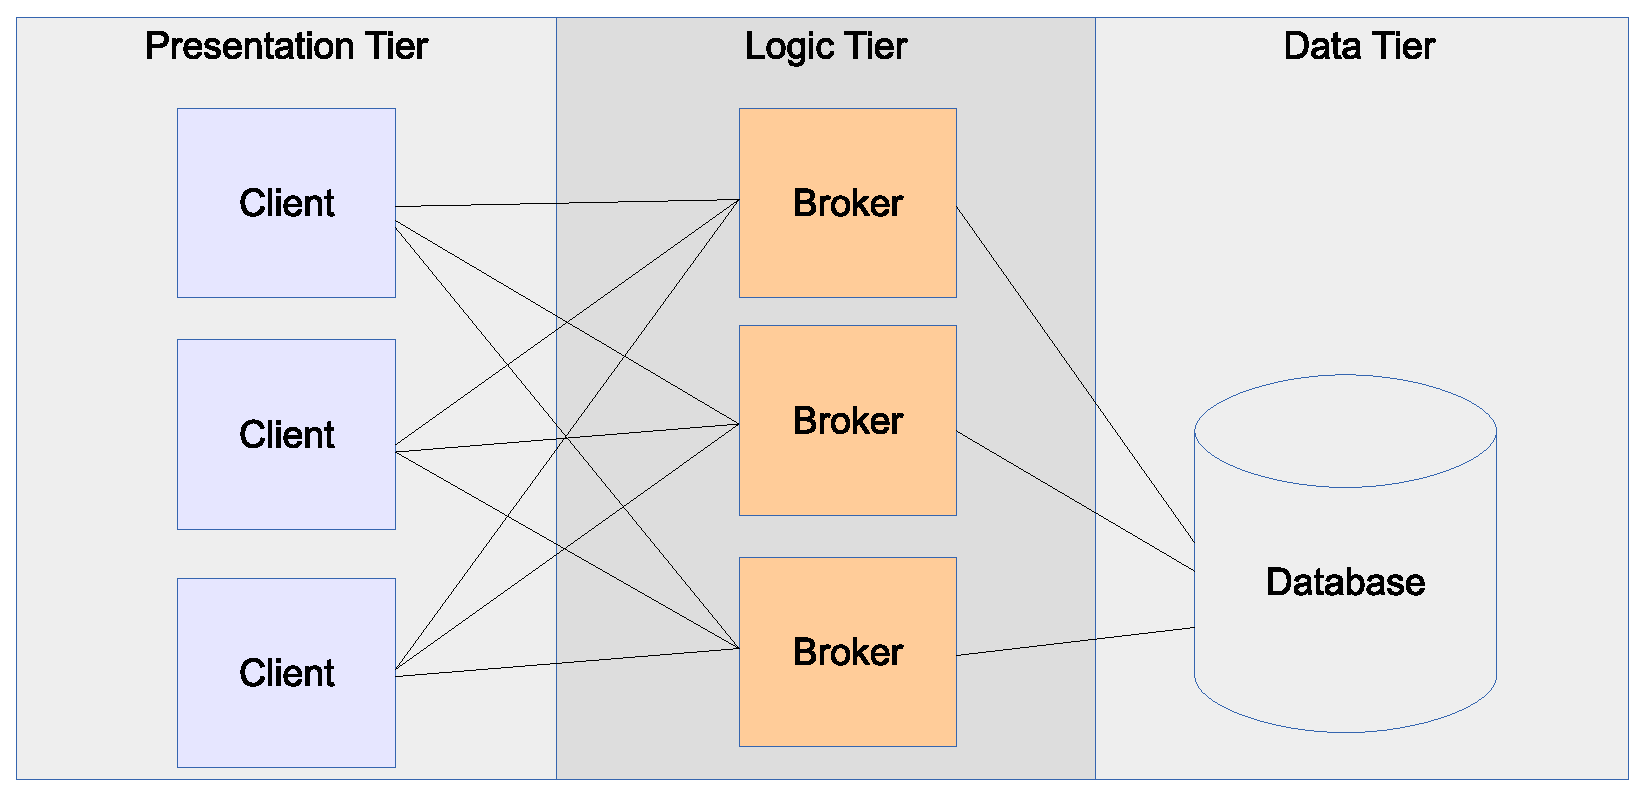
\includegraphics[scale=0.4]{../drawings/system-overview.eps}
  \end{center}
  \caption{System Overview}
  \label{fig:system-overview}
\end{figure}

Figure \ref{fig:middleware-threading} shows important software components of a single middle ware. A nonblocking network interface (NIO) handles communication to the clients. Received data is put to a single thread safe request queue.

A configurable number of workers are constantly reading from the request queue. As soon as a worker gets a piece of work (request raw data) it then performs the following tasks:
\begin{itemize}
\item decoding: The raw request is parsed and converted into a request java object
\item process: The request is processes. The database is accesses and a response object is created
\item encode: The response object is serialized and placed into the response queue of the network interface.
\end{itemize}

% ------------------------------------------------
% Figure - threading

\begin{figure}
	\begin{center}
    \includegraphics[scale=0.4]{../drawings/broker-threading.eps}
  \end{center}
  \caption{Middleware's main Components}
  \label{fig:middleware-threading}
\end{figure}

%% ----------------------------------------------
% Section Design Decisions
%% ----------------------------------------------
\subfile{part02-design.tex}


%% ----------------------------------------------
% Section Performance Relevant Features
%% ----------------------------------------------
\subfile{part03-features.tex}

%% ----------------------------------------------
% Section Experiments
%% ----------------------------------------------
\subfile{part04-experiments.tex}

%% ----------------------------------------------
% Section How to Run the system
%% ----------------------------------------------

\section{How to run the System}

This section describe all the important things laying around the core messaging system.

\subsection{Database setup}

To setup the database required for the middle ware there are 2 option
how to setup the database

\subsubsection{Automatic setup}
You can run the java class \textit{ch.ethz.mlmq.main.Main} which is located in the main project folder \textit{mlmq}. Run the class without parameters to get usage informations.

Sample Start parameters may look like this:

\begin{verbatim} 
java ch.ethz.mlmq.main.Main dbscript -url jdbc:postgresql://localhost:5432 -db mlmq -user myusername -password mypassword -createDatabase -createTables
\end{verbatim}

\subsubsection{Manual setup}
Use your favourite database management tool (pgadmin) and execute the following sql scripts which can be found here:

\begin{verbatim} 
resource/db/001_table_create.sql
resource/db/002_stored_procedures.sql
\end{verbatim}

\subsection{Configuration}

\subsubsection{Main Configuration}
\label{subsub:MainConfig}

Have a look at the example configuration located at the following place.

\begin{verbatim} 
resource/config.example.properties
\end{verbatim}

Most of the configuration should be self explanatory. An exception may be the the part which is dynamically generated part when executed via test infrastructure (see figure \ref{fig:SampleConfig}). This part of the configuration describes the configuration of an experiment.

\begin{verbatim} 
common.scenario.mytype
\end{verbatim}
Describes whether this configuration file belongs to a client or a middle ware instance.

\begin{verbatim} 
common.scenario.myposition = n
\end{verbatim}
Together with \textit{common.scenario.mytype} it determines whether to pick the n-th configuration from\textit{ common.scenario.mapping.broker} or \textit{common.scenarion.mapping.client}.

\begin{verbatim} 
common.scenario.mapping.broker=...
\end{verbatim}
Lists the Broker scenarios to use. Where the first item corresponds to a class name followed by ip address and port

\begin{verbatim} 
common.scenario.mapping.client=...
\end{verbatim}
Lists the client scenarios to use. Where the first item corresponds to a class name followed by ip address

\begin{figure}
\begin{verbatim} 

...

##################################################
# Dynamically generated per test run from here on
##################################################

...

# Scenario mapping format: name1:ip,ip,ip,...;name2:ip,ip,...;name3:ip,ip,...
# E.g. scenario.mapping = broker:127.0.0.1,192.168.0.2;client:127.0.0.1,192.168.0.1
# Here: only one broker and one client
common.scenario.mapping.broker = SimpleShutdownBroker#127.0.0.1:8099;SimpleShutdownBroker#127.0.0.1:8100,127.0.0.1:8101
common.scenario.mapping.client = SimpleSendClient#127.0.0.1;SimpleSendClient#127.0.0.1;SimpleSendClient#127.0.0.1;SimpleSendClient#127.0.0.1,127.0.0.1

# either broker or client
common.scenario.mytype = client

# If the position is 5 and mytype is a broker, then this means that this is the 5th broker
# myposition starts at position 0
common.scenario.myposition = 0

...

\end{verbatim}
\caption{Sample Config}
\label{fig:SampleConfig}
\end{figure}  	

\subsubsection{Logging Configuration}

Both the messaging system and the client implementation use \textit{java.util.logging.*} to log system events like errors, component startup/shutdown. This log is completely separated from the performance log (see \ref{subsub:PerfLogConfig} ), which is performed on a separate basis.

A valid logging configuration can be found here

\begin{verbatim} 
resource/logging.properties
\end{verbatim}

\subsubsection{Performance Logging Configuration}
\label{subsub:PerfLogConfig}

As already state performance logging is separated from the default logging. Any activity which may be interesting to measure is logged via this performance logger. This logger is configured via the main configuration file (see \ref{subsub:MainConfig}) and is kept simple. You just specify a path where the performance logger puts the file

\begin{verbatim} 
# folder where to write the performance log
common.performancelogger.logfilepath = performance_log
\end{verbatim}

\subsection{Start a Middleware instance/Client}
As soon as both main and logging configuration files are prepared starting the middle ware instance is easy. Just specify both files via command line arguments like the following:

\begin{verbatim} 
java ch.ethz.mlmq.main.Main scenario -config resource/brokerconfig.properties -l resource/logging.properties
\end{verbatim}

Since configuration whether to start as a client or as a server is located inside the main configuration file a client is started in the same way as a middle ware.

\subsection{Command Line Interface}
command line interface commando file

\subsection{Logging}
what has been logged
performance logger
how to configure logging


\subsection{Unit Tests}
unit tests
system tests
what do they do


\section{Test Infrastructure}
describe the testmaster
\subsection{Overview}
what we've built
what it does

\subsection{How to set up a test}
describe the web GUI

\subsection{Log Analyzer}
describe the log analyzer



%% ----------------------------------------------
% Section References
%% ----------------------------------------------
\section{References}

% TODO

http://dl.acm.org/citation.cfm?id=SERIES12798.1557393

@book{hanmer2007patterns,
  title={Patterns for fault tolerant software},
  author={Hanmer, Robert},
  year={2007},
  isbn = {0470319798, 9780470319796},
  publisher={Wiley Publishing}
}

%\bibliography{mybib}

%% %%%%%%%%%%%%%%%%%%%%%%%%%%%%%%%%%%%%%%%%%%%%%%%%%%%%%%%%%%%%%%%%%%%%%%%%%
\section{Notes - to delete}

% unit test

\subsection{What should be included in this report }

\subsubsection{System Code}
\begin{itemize}
\item Code
\item Scripts for experiment
\end{itemize}

\subsubsection{Experimental data}
\begin{itemize}
\item Basic tests ans simple traces
\item Long running traces, Raw data and graphs for all experiments
\end{itemize}

\subsubsection{Written report}
\begin{itemize}
\item Architectural  diagrams
\item Interface description
\item explanation of the system design
\item Description of all experiments
\item statistical treatment of data
\item commentary analysis
\end{itemize}


\end{document}
